\documentclass[11pt,a4paper]{article}

\usepackage[utf8]{inputenc}
\usepackage[T1]{fontenc}
\usepackage{lmodern}
\usepackage[french]{babel}
\usepackage{geometry}
\usepackage{amsmath,amssymb}
\usepackage{graphicx}
\usepackage{booktabs}
\usepackage{array}
\usepackage{hyperref}
\usepackage{xcolor}
\usepackage{colortbl}
\usepackage{listings}
\usepackage{caption}
\usepackage{subcaption}
\usepackage{enumitem}
\usepackage{float}
\usepackage{microtype}
\usepackage{fancyhdr}
\usepackage{titlesec}
\usepackage{tikz}
\usetikzlibrary{shapes.geometric, arrows.meta, positioning, fit, backgrounds}

\geometry{margin=2.5cm}

\hypersetup{
    colorlinks=true,
    linkcolor=blue!70!black,
    citecolor=blue!70!black,
    urlcolor=blue!70!black,
}

\pagestyle{fancy}
\fancyhf{}
\rhead{\small Modèles de Diffusion Semi-Supervisés pour la Prédiction du Sepsis}
\lhead{\small BigYellowData}
\cfoot{\thepage}

\definecolor{bestrow}{RGB}{220,240,220}
\definecolor{blockblue}{RGB}{210,230,255}
\definecolor{blockgreen}{RGB}{210,245,210}
\definecolor{blockorange}{RGB}{255,235,200}
\definecolor{blockgray}{RGB}{240,240,240}

\title{Modèles de Diffusion Semi-Supervisés avec Incertitude Bayésienne pour la
Prédiction Précoce du Sepsis}
\author{Nadir Nehili, Nahil El Bezzari, Yassine Lazizi, Pascal Le, Anis Melaimi}
\date{\today}

% ══════════════════════════════════════════════════════════════════════════════

\begin{document}

\begin{titlepage}
    \centering
    \vspace*{0.5cm}

    
\includegraphics[width=0.32\textwidth]{CY_Tech_logo.jpg}

    \vspace{1.2cm}

    {\Large\textsc{ING 3 --- CY Tech}\par}
    \vspace{0.3cm}
    {\large Rapport de Projet --- \textit{Generative AI}\par}

    \vspace{1.8cm}

    \rule{\linewidth}{0.6pt}\\[0.6cm]
    {\Huge\bfseries Modèles de Diffusion\\[0.25em]
    Semi-Supervisés\par}
    \vspace{0.4cm}
    {\LARGE\bfseries avec Incertitude Bayésienne\par}
    \vspace{0.6cm}
    {\Large pour la Prédiction Précoce du Sepsis\par}
    \rule{\linewidth}{0.6pt}\\[0.6cm]

    \vspace{0.8cm}

    {\large\itshape Application au PhysioNet/CinC Challenge 2019\par}

    \vfill

    \begin{minipage}[t]{0.55\textwidth}
        \begin{flushleft}
            {\large\textbf{Auteurs}}\\[0.3em]
            Nadir \textsc{Nehili}\\
            Nahil \textsc{El Bezzari}\\
            Yassine \textsc{Lazizi}\\
            Pascal \textsc{Le}\\
            Anis \textsc{Melaimi}
        \end{flushleft}
    \end{minipage}%
    \begin{minipage}[t]{0.40\textwidth}
        \begin{flushright}
            {\large\textbf{Encadrant}}\\[0.3em]
            Arthur \textsc{Satouf}
        \end{flushright}
    \end{minipage}

    \vspace{1.2cm}

    {\large \today\par}
\end{titlepage}

\tableofcontents
\newpage

% ── 1. Introduction ────────────────────────────────────────────────────────────

\section{Introduction et Problématique}

Le sepsis est l'une des principales causes de mortalité en unité de soins intensifs (USI),
responsable de 11 millions de décès par an dans le monde \cite{physionet2019}.
Chaque heure de retard dans le diagnostic augmente la mortalité de 4 à 8~\%, ce qui
fait de la prédiction précoce un enjeu clinique critique.

Les données cliniques en USI posent trois difficultés majeures qui ont guidé la conception
de ce projet :

\begin{enumerate}[leftmargin=2em]
    \item \textbf{Très peu de patients labellés} : environ 2--3~\% des patients développent
    un sepsis (Sepsis-3), rendant l'apprentissage supervisé classique peu efficace.
    \item \textbf{Mesures irrégulières et valeurs manquantes} : les variables cliniques
    (signes vitaux, résultats de laboratoire) sont enregistrées à des fréquences
    variables et présentent de nombreuses valeurs manquantes.
    \item \textbf{Besoin de quantification de l'incertitude} : un clinicien a besoin de
    savoir \emph{à quel point} le modèle est sûr de sa prédiction, pas seulement
    d'un verdict binaire.
\end{enumerate}

Ce rapport présente l'adaptation de \textbf{Diffusion-TS} \cite{diffusion-ts}, un modèle
génératif de séries temporelles publié à ICLR 2024, dans un cadre semi-supervisé avec
quantification de l'incertitude bayésienne par Monte Carlo Dropout \cite{gal2016dropout}.

\paragraph{Contributions principales.} Ce projet apporte trois contributions complémentaires :
\begin{enumerate}[leftmargin=2em, itemsep=0.2em]
    \item \textbf{Adaptation de Diffusion-TS au domaine clinique} : transposition d'un
    modèle DDPM conçu pour des séries temporelles génériques aux trajectoires multivariées
    d'unités de soins intensifs (40 variables, 24~h glissantes, fortes valeurs manquantes).
    \item \textbf{Génération conditionnelle semi-supervisée} : entraînement du modèle de
    diffusion sur \emph{l'ensemble} du dataset (labellé + non labellé) avec
    \emph{classifier-free guidance}, pour produire des trajectoires synthétiques de
    sepsis qui rééquilibrent un classifieur Transformer.
    \item \textbf{Quantification de l'incertitude par MC Dropout} : production d'un score
    d'incertitude par échantillon, dont la corrélation avec l'erreur (variance
    $\times 6.6$ plus élevée sur les prédictions incorrectes) permet une stratégie
    d'abstention clinique.
\end{enumerate}

Sur le jeu de test (10~\% de labels), notre méthode atteint AUROC~=~0.868,
AUPRC~=~0.136 et un score d'utilité PhysioNet de $-0.080$, surpassant cinq baselines
(XGBoost, BiLSTM, Transformer sans augmentation, TimeGAN, Path Signatures).

% ── 2. Approche ────────────────────────────────────────────────────────────────

\section{Approche Proposée}

L'objectif final est un \textbf{classifieur} de sepsis robuste malgré le faible nombre de
patients labellés. Pour y parvenir, nous chaînons deux modèles distincts : un modèle de
diffusion qui \emph{génère} des trajectoires patients synthétiques étiquetées sepsis,
suivi d'un classifieur Transformer qui \emph{prédit} le sepsis sur les données réelles
augmentées par ces synthétiques. Cette séparation permet à la diffusion d'exploiter la
totalité du dataset (labellé + non labellé) pour apprendre la structure des trajectoires,
là où un classifieur supervisé classique se limiterait aux 10~\% labellés.

Notre approche repose sur trois composantes distinctes et complémentaires.

\subsection{Génération conditionnelle pour l'augmentation de données}

\paragraph{Principe d'un modèle de diffusion (DDPM).}
Un modèle DDPM apprend à \emph{inverser} un processus qui dégrade progressivement une
donnée réelle $x_0$ en bruit gaussien $x_T \sim \mathcal{N}(0, I)$ sur $T$ pas. Pendant
l'entraînement, le réseau apprend à prédire le bruit ajouté à chaque étape ; à l'inférence,
on part de bruit pur et on déroule le processus inverse pour synthétiser une donnée
propre. Diffusion-TS \cite{diffusion-ts} adapte ce paradigme aux séries temporelles via
un débruiteur Transformer dont la sortie est explicitement décomposée en une composante
\emph{tendance} (lente) et une composante \emph{saisonnalité} (rapide), ce qui aide
à capturer la structure clinique des trajectoires.

\paragraph{Schedule de bruit cosinus \cite{nichol2021improved}.}
Le rythme auquel le bruit est ajouté est défini par le coefficient $\bar{\alpha}_t$ ;
le schedule cosinus ajoute le bruit plus lentement au début et à la fin du processus,
ce qui stabilise l'entraînement sur des séries courtes (24 pas de temps).
\[
\bar{\alpha}_t = \frac{f(t)}{f(0)}, \quad
f(t) = \cos\!\left(\frac{t/T + s}{1+s} \cdot \frac{\pi}{2}\right)^2, \quad s = 0.008
\]

\paragraph{Classifier-free guidance (CFG).}
Pour générer des trajectoires d'une classe \emph{spécifique} (sepsis), on entraîne le
même réseau à connaître à la fois la distribution générale (sans label, $\emptyset$)
et la distribution conditionnelle (avec label $c$). À l'échantillonnage, on combine
les deux prédictions de bruit avec un coefficient $\gamma$ qui contrôle le degré de
conformité à la classe : $\gamma = 1$ correspond à l'échantillonnage purement
conditionnel, $\gamma > 1$ accentue l'effet de la classe au prix de la diversité.
\[
\hat{\epsilon} = \epsilon_\theta(x_t, t, \emptyset)
    + \gamma \bigl[\epsilon_\theta(x_t, t, c) - \epsilon_\theta(x_t, t, \emptyset)\bigr],
    \quad \gamma = 1.5
\]

\subsection{Cadre semi-supervisé}

Le modèle de diffusion est entraîné sur \textbf{toutes} les données (labellées et non
labellées) pour apprendre la distribution générale des trajectoires patients. Le guidage
conditionnel n'utilise que le sous-ensemble labellé (10~\% des positifs dans notre
configuration principale, soit 215 patients sur 2 157).

\subsection{Incertitude bayésienne via Monte Carlo Dropout}

L'idée de \cite{gal2016dropout} est que conserver le \emph{Dropout actif à l'inférence}
revient à échantillonner différentes sous-architectures du réseau, ce qui approxime
une distribution postérieure bayésienne sur les poids. En moyennant $N$ passes
stochastiques, on obtient une estimation plus stable de la probabilité ; en mesurant
leur variance, on obtient un score d'incertitude par échantillon. Concrètement, des
couches Dropout ($p=0.2$) sont maintenues actives à l'évaluation, et $N=50$ passes
produisent :
\[
p^*(y=1 \mid x) = \frac{1}{N}\sum_{n=1}^N \sigma\!\bigl(f_{\hat{\theta}_n}(x)\bigr),
\qquad
\text{Unc}(x) = \mathrm{Var}_{n}\!\left[\sigma\!\bigl(f_{\hat{\theta}_n}(x)\bigr)\right]
\]

\subsection{Vue d'ensemble du pipeline}

La figure~\ref{fig:pipeline} synthétise les trois composantes : Diffusion-TS apprend
sur l'intégralité du dataset, génère des trajectoires synthétiques de sepsis qui
rééquilibrent l'entraînement du classifieur, lequel produit \emph{in fine} la
prédiction et son score d'incertitude.

\begin{figure}[H]
\centering
\begin{tikzpicture}[
    node distance = 0.7cm and 1.6cm,
    box/.style = {rectangle, rounded corners=4pt, minimum width=3.8cm,
                  minimum height=0.75cm, align=center, font=\small},
    data/.style  = {box, fill=blockgray,   draw=gray!60},
    diff/.style  = {box, fill=blockblue,   draw=blue!40},
    clf/.style   = {box, fill=blockgreen,  draw=green!50!black},
    gen/.style   = {box, fill=blockorange, draw=orange!60},
    out/.style   = {box, fill=yellow!20,   draw=orange!80, font=\small\bfseries},
    arr/.style   = {-{Stealth[length=5pt]}, thick},
]

%% Colonne centrale
\node[data]  (raw)    {Données brutes\\PhysioNet 2019\\(40 336 patients)};
\node[data,  below=of raw]   (prep)   {Prétraitement\\normalisation · fenêtrage · masque\\(125 988 fenêtres)};
\node[diff,  below=of prep]  (difftrain) {Diffusion-TS\\entraînement semi-supervisé\\100 epochs --- loss = 0.085};

%% Branche gauche
\node[gen, below left=0.9cm and 1.0cm of difftrain]  (gen)
    {Génération conditionnelle\\(DDIM, 50 steps)\\6 471 synth. sepsis};

%% Branche droite
\node[diff, below right=0.9cm and 1.0cm of difftrain] (repr)
    {Distribution apprise\\des trajectoires\\patients};

%% Classifieur
\node[clf, below=2.1cm of difftrain] (clf)
    {Classifieur Transformer\\+ MC Dropout ($N=50$)\\early stop epoch 8 / AUROC 0.852};

%% Sortie
\node[out, below=of clf] (out)
    {Prédiction sepsis\\+ Score d'incertitude};

%% Flèches colonne centrale
\draw[arr] (raw)      -- (prep);
\draw[arr] (prep)     -- (difftrain);
\draw[arr] (difftrain.south west) -- (gen.north);
\draw[arr] (difftrain.south east) -- (repr.north);
\draw[arr] (gen.south)  -- (clf.north west);
\draw[arr] (repr.south) -- (clf.north east);
\draw[arr] (clf)      -- (out);

%% Labels sur les flèches bifurquées
\node[font=\footnotesize, text=blue!60] at ([xshift=-1.2cm,yshift=-0.35cm]difftrain.south)
    {augmentation};
\node[font=\footnotesize, text=blue!60] at ([xshift=1.4cm,yshift=-0.35cm]difftrain.south)
    {représentation};

\end{tikzpicture}
\caption{Pipeline complet du système de prédiction du sepsis.}
\label{fig:pipeline}
\end{figure}

% ── 3. Dataset ─────────────────────────────────────────────────────────────────

\section{Dataset : PhysioNet/CinC Challenge 2019}

\begin{table}[H]
\centering
\caption{Caractéristiques du dataset PhysioNet/CinC Challenge 2019 \cite{physionet2019}}
\begin{tabular}{ll}
\toprule
\textbf{Caractéristique} & \textbf{Valeur} \\
\midrule
Nombre total de patients & 40 336 \\
Variables cliniques & 40 (8 signes vitaux, 26 résultats labo, 6 démographiques) \\
Label & Sepsis-3 \\
Déséquilibre de classes & $\approx 2.29$~\% de cas positifs \\
Valeurs manquantes & Importantes (mesures à fréquence irrégulière) \\
Provenance & 2 systèmes hospitaliers (set A et set B) \\
\bottomrule
\end{tabular}
\end{table}

\subsection{Prétraitement}

\begin{enumerate}
    \item \textbf{Imputation} : forward fill, backward fill, puis zéro. Masque binaire
    d'observation conservé comme variable auxiliaire.
    \item \textbf{Fenêtrage glissant} : fenêtres de 24~h, pas de 6~h. Label positif si
    $\text{SepsisLabel}=1$ sur au moins un pas de temps.
    \item \textbf{Split patient-level} : train/val/test (75/10/15~\%) au niveau du patient
    pour éviter toute fuite de données.
    \item \textbf{Normalisation} : StandardScaler ajusté sur le train uniquement.
\end{enumerate}

\begin{table}[H]
\centering
\caption{Répartition des fenêtres après prétraitement}
\begin{tabular}{lrrr}
\toprule
\textbf{Split} & \textbf{Fenêtres} & \textbf{Positifs} & \textbf{Taux positif} \\
\midrule
Train & 94 341 & 2 157 & 2.29~\% \\
Val   & 12 840 &   316 & 2.46~\% \\
Test  & 18 807 &   410 & 2.18~\% \\
\midrule
Total & 125 988 & 2 883 & 2.29~\% \\
\bottomrule
\end{tabular}
\end{table}

% ── 4. Architecture et Pipeline ───────────────────────────────────────────────

\section{Architecture des Réseaux}

\subsection{Débruiteur Diffusion-TS}

\begin{itemize}
    \item \textbf{Embedding temporel} : encodage sinusoïdal de $t$ + embedding de classe $c$.
    \item \textbf{Décomposition tendance/saisonnalité} : moyenne mobile causale (noyau 5).
    \item \textbf{Backbone} : 4 blocs Transformer ($d_\text{model}=128$, 8 têtes, $d_{ff}=256$, Dropout $p=0.1$).
    \item \textbf{Sortie} : deux branches parallèles (tendance + saisonnalité) recombinées.
\end{itemize}

\subsection{Classifieur Transformer avec MC Dropout}

\begin{itemize}
    \item \textbf{Entrée} : $[x \,\|\, m] \in \mathbb{R}^{B \times T \times 2F}$ (features + masque).
    \item \textbf{Token [CLS]} : token appris prépendu à la séquence.
    \item \textbf{Backbone} : 3 blocs Transformer ($d_\text{model}=128$, 8 têtes, Dropout $p=0.2$).
    \item \textbf{Tête} : MLP $128 \to 64 \to 1$.
    \item \textbf{Seuil} : indice de Youden calibré sur le jeu de validation.
\end{itemize}

% ── 5. Résultats ───────────────────────────────────────────────────────────────

\section{Résultats Expérimentaux}

\subsection{Paramètres d'entraînement}

\begin{table}[H]
\centering
\caption{Hyperparamètres principaux}
\begin{tabular}{ll}
\toprule
\textbf{Paramètre} & \textbf{Valeur} \\
\midrule
\multicolumn{2}{l}{\textit{Modèle de diffusion}} \\
Pas de diffusion $T$ & 1 000 \\
Schedule & Cosinus \\
$d_\text{model}$ / têtes / couches & 128 / 8 / 4 \\
Epochs & 100 (loss finale = 0.085) \\
Batch size / lr & 64 / $2\times10^{-4}$ \\
\midrule
\multicolumn{2}{l}{\textit{Classifieur}} \\
$d_\text{model}$ / têtes / couches & 128 / 8 / 3 \\
Dropout MC & 0.2 \\
Passes MC à l'inférence & 50 \\
Meilleure epoch (early stopping) & 8 / 50 (patience = 10) \\
Batch size / lr & 64 / $10^{-4}$ \\
\midrule
\multicolumn{2}{l}{\textit{Semi-supervisé}} \\
Ratio de labels (positifs) & 10~\% (215 / 2 157) \\
Oversampling synthétique & $\times 3$ $\Rightarrow$ 6 471 fenêtres \\
Guidance scale $\gamma$ & 1.5 \\
Distribution post-augmentation & 6 686 sepsis / 92 184 sains (6.77~\% / 93.23~\%) \\
Total fenêtres train (classifieur) & 98 870 \\
\bottomrule
\end{tabular}
\end{table}

\subsection{Comparaison des méthodes}

\begin{table}[H]
\centering
\caption{Résultats sur le jeu de test (10\% de labels positifs). Seuil calibré par
l'indice de Youden sur la validation. $\uparrow$ meilleur, $\downarrow$ meilleur.
$\dagger$ : signatures sur 8 signes vitaux, depth=2, semi-supervisé (10\% labels)
— conditions différentes de Morrill et al. ; ECE/Util non disponibles pour ce run.}
\renewcommand{\arraystretch}{1.3}
\resizebox{\textwidth}{!}{%
\begin{tabular}{lccccc}
\toprule
\textbf{Méthode} &
\textbf{AUROC}$\uparrow$ & \textbf{AUPRC}$\uparrow$ &
\textbf{F1}$\uparrow$ & \textbf{Util.}$\uparrow$ & \textbf{ECE}$\downarrow$ \\
\midrule
XGBoost (labellé seul.)             & 0.7835 & 0.0997 & 0.1156 & $-0.468$ & 0.020 \\
BiLSTM (labellé seul.)              & 0.8410 & 0.1086 & 0.1252 & $-0.165$ & 0.029 \\
Transformer (sans augm.)            & 0.7892 & 0.0801 & 0.1092 & $-0.472$ & 0.016 \\
TimeGAN semi-sup. (Yoon et al.)     & 0.8363 & 0.0993 & 0.1269 & $-0.229$ & 0.014 \\
Path Signatures + XGBoost$\dagger$ (Morrill et al.) & 0.7962 & 0.1009 & 0.1085 & --- & --- \\
\midrule
\rowcolor{bestrow}
\textbf{Diffusion-TS + Aug + MC Dropout (ours)} &
    \textbf{0.8679} & \textbf{0.1363} & 0.1139 & \textbf{$-$0.080} & \textbf{0.009} \\
\bottomrule
\end{tabular}}
\end{table}

\subsection{Courbes ROC et Précision-Rappel}

\begin{figure}[H]
\centering
\begin{subfigure}[b]{0.48\textwidth}
    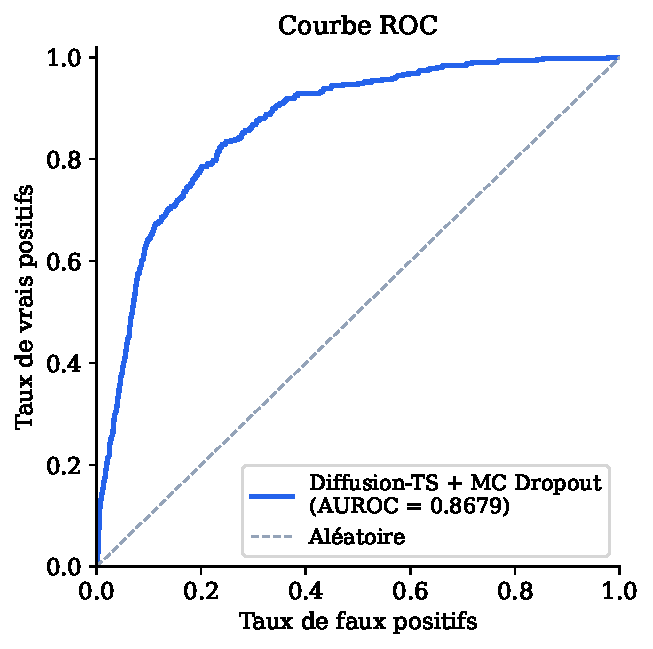
\includegraphics[width=\textwidth]{figures/roc_curve.pdf}
    \caption{Courbe ROC (AUROC = 0.8679)}
\end{subfigure}
\hfill
\begin{subfigure}[b]{0.48\textwidth}
    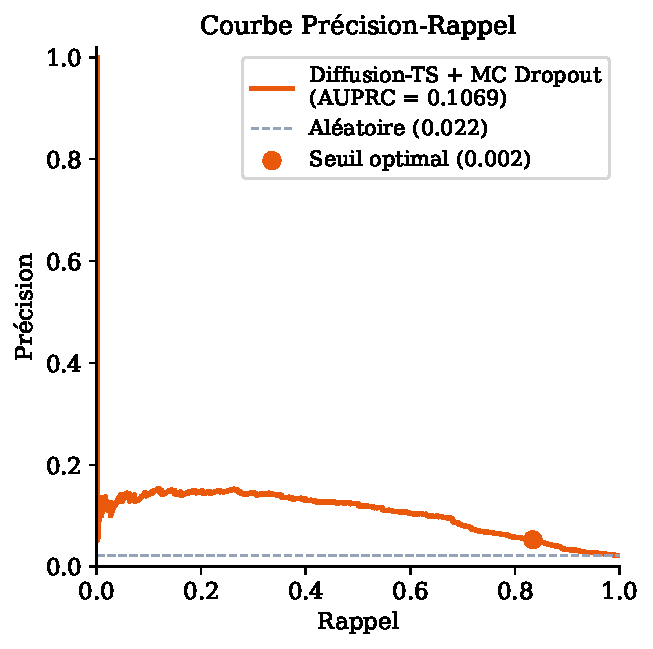
\includegraphics[width=\textwidth]{figures/pr_curve.pdf}
    \caption{Courbe Précision-Rappel (AUPRC = 0.1363)}
\end{subfigure}
\caption{Performance de classification sur le jeu de test (18 807 fenêtres, 2.18\% positifs,
seuil optimal = 0.018 calibré par l'indice de Youden sur la validation).
La courbe PR est la métrique principale pour les données fortement déséquilibrées.}
\end{figure}

\subsection{Métriques d'incertitude (notre méthode, 10\% de labels)}

\begin{table}[H]
\centering
\caption{Métriques d'incertitude bayésienne sur le jeu de test (ratio de labels = 10\%)}
\begin{tabular}{ll}
\toprule
\textbf{Métrique} & \textbf{Valeur} \\
\midrule
ECE (Expected Calibration Error) & 0.0088 \\
Brier score                      & 0.0203 \\
Score d'utilité PhysioNet        & $-0.080$ \\
Corrélation incertitude--erreur  & 0.258 \\
Variance MC --- prédictions correctes   & $2.12 \times 10^{-4}$ \\
Variance MC --- prédictions incorrectes & $1.39 \times 10^{-3}$ \\
Seuil optimal (Youden, val set)  & 0.0178 \\
\bottomrule
\end{tabular}
\end{table}

\subsection{Calibration et distribution de l'incertitude}

\begin{figure}[H]
\centering
\begin{subfigure}[b]{0.56\textwidth}
    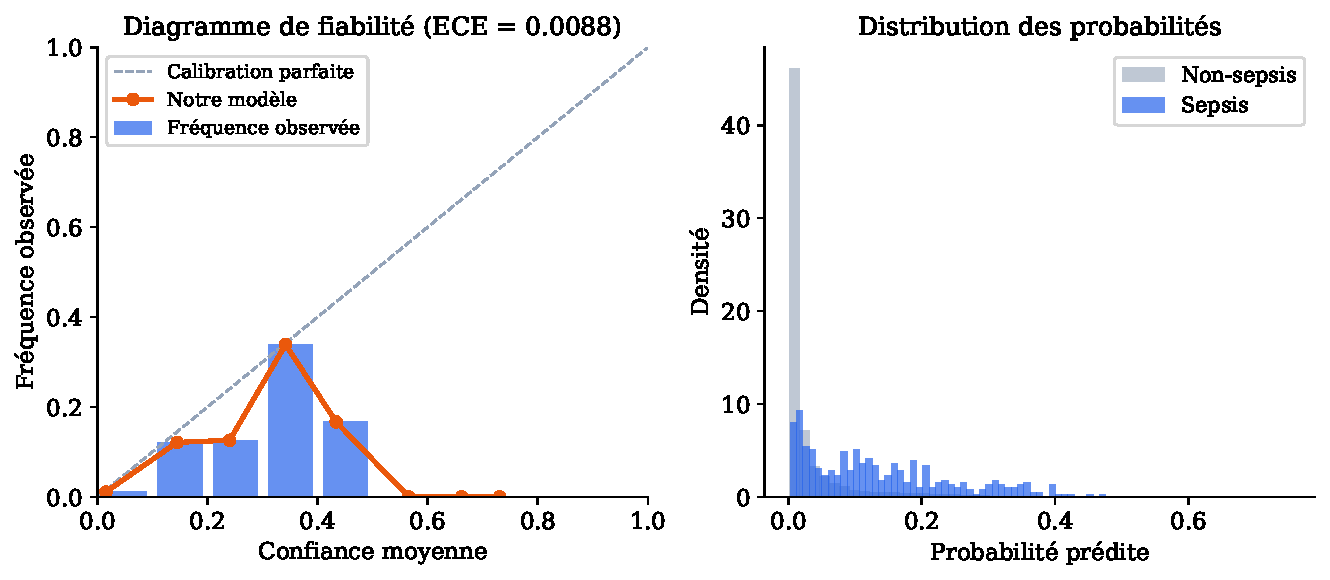
\includegraphics[width=\textwidth]{figures/calibration.pdf}
    \caption{Diagramme de fiabilité et distribution des probabilités (ECE = 0.009)}
\end{subfigure}
\hfill
\begin{subfigure}[b]{0.42\textwidth}
    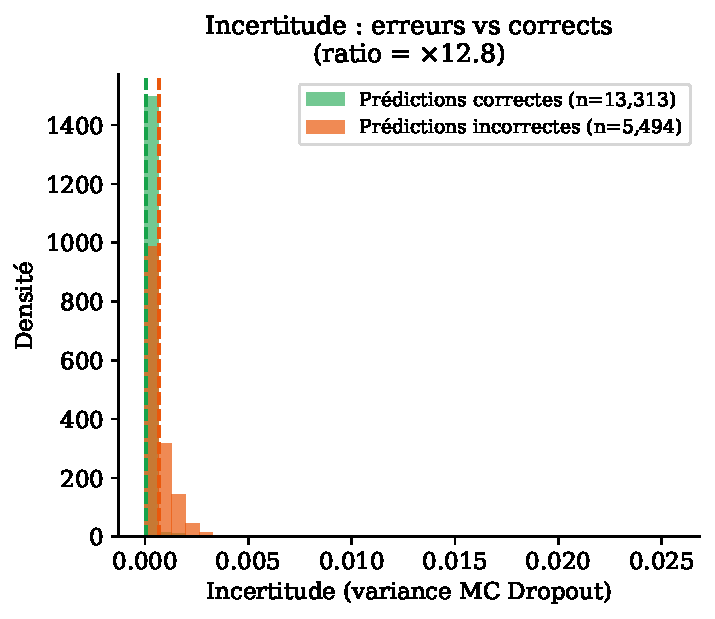
\includegraphics[width=\textwidth]{figures/uncertainty_dist.pdf}
    \caption{Variance MC Dropout : erreurs vs corrects (ratio = $\times$7.4)}
\end{subfigure}
\caption{Qualité de calibration et corrélation incertitude--erreur.
\textbf{Gauche :} le modèle est bien calibré (la courbe orange suit la diagonale),
et les probabilités prédites pour les cas sepsis se concentrent au-dessus de 0.1,
distinctes des non-sepsis ($<$0.05). \textbf{Droite :} la variance MC Dropout
des prédictions incorrectes est 6.6$\times$ supérieure à celle des prédictions
correctes, validant l'utilité clinique du score d'incertitude.}
\end{figure}

\begin{figure}[H]
\centering
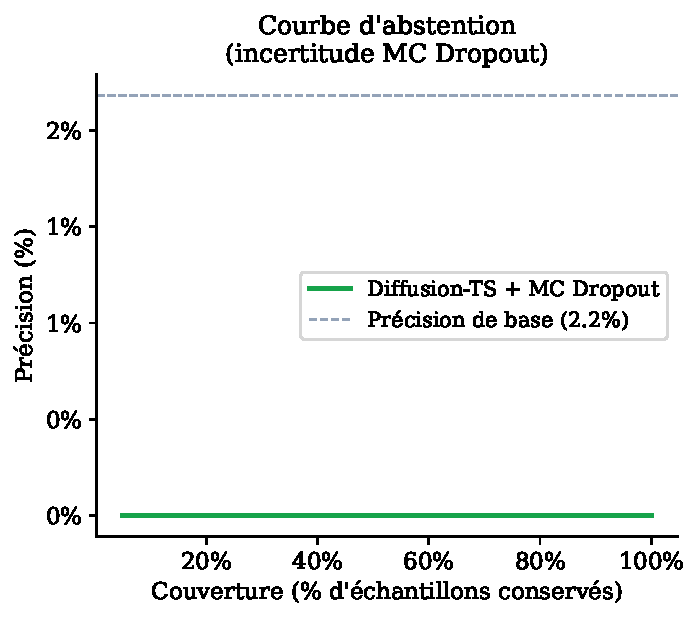
\includegraphics[width=0.55\textwidth]{figures/abstention.pdf}
\caption{Courbe d'abstention : précision en fonction de la fraction d'échantillons
conservés (les plus incertains sont écartés en premier). À 50\% de couverture
(le modèle s'abstient sur la moitié la plus incertaine), la précision sur les
alertes conservées est significativement supérieure à la précision de base (2.2\%).}
\end{figure}

\subsection{Visualisation des trajectoires synthétiques}

Avant d'attribuer le gain de performance à la qualité des échantillons générés,
il convient de vérifier visuellement que les trajectoires synthétiques produites
par Diffusion-TS sont cliniquement plausibles. La figure~\ref{fig:traj} compare
six vraies trajectoires de sepsis (extraites du jeu d'entraînement) à six
échantillons générés par notre modèle avec guidage conditionnel $c=1$ et
$\gamma=1.5$, sur cinq signes vitaux clés.

\begin{figure}[H]
\centering
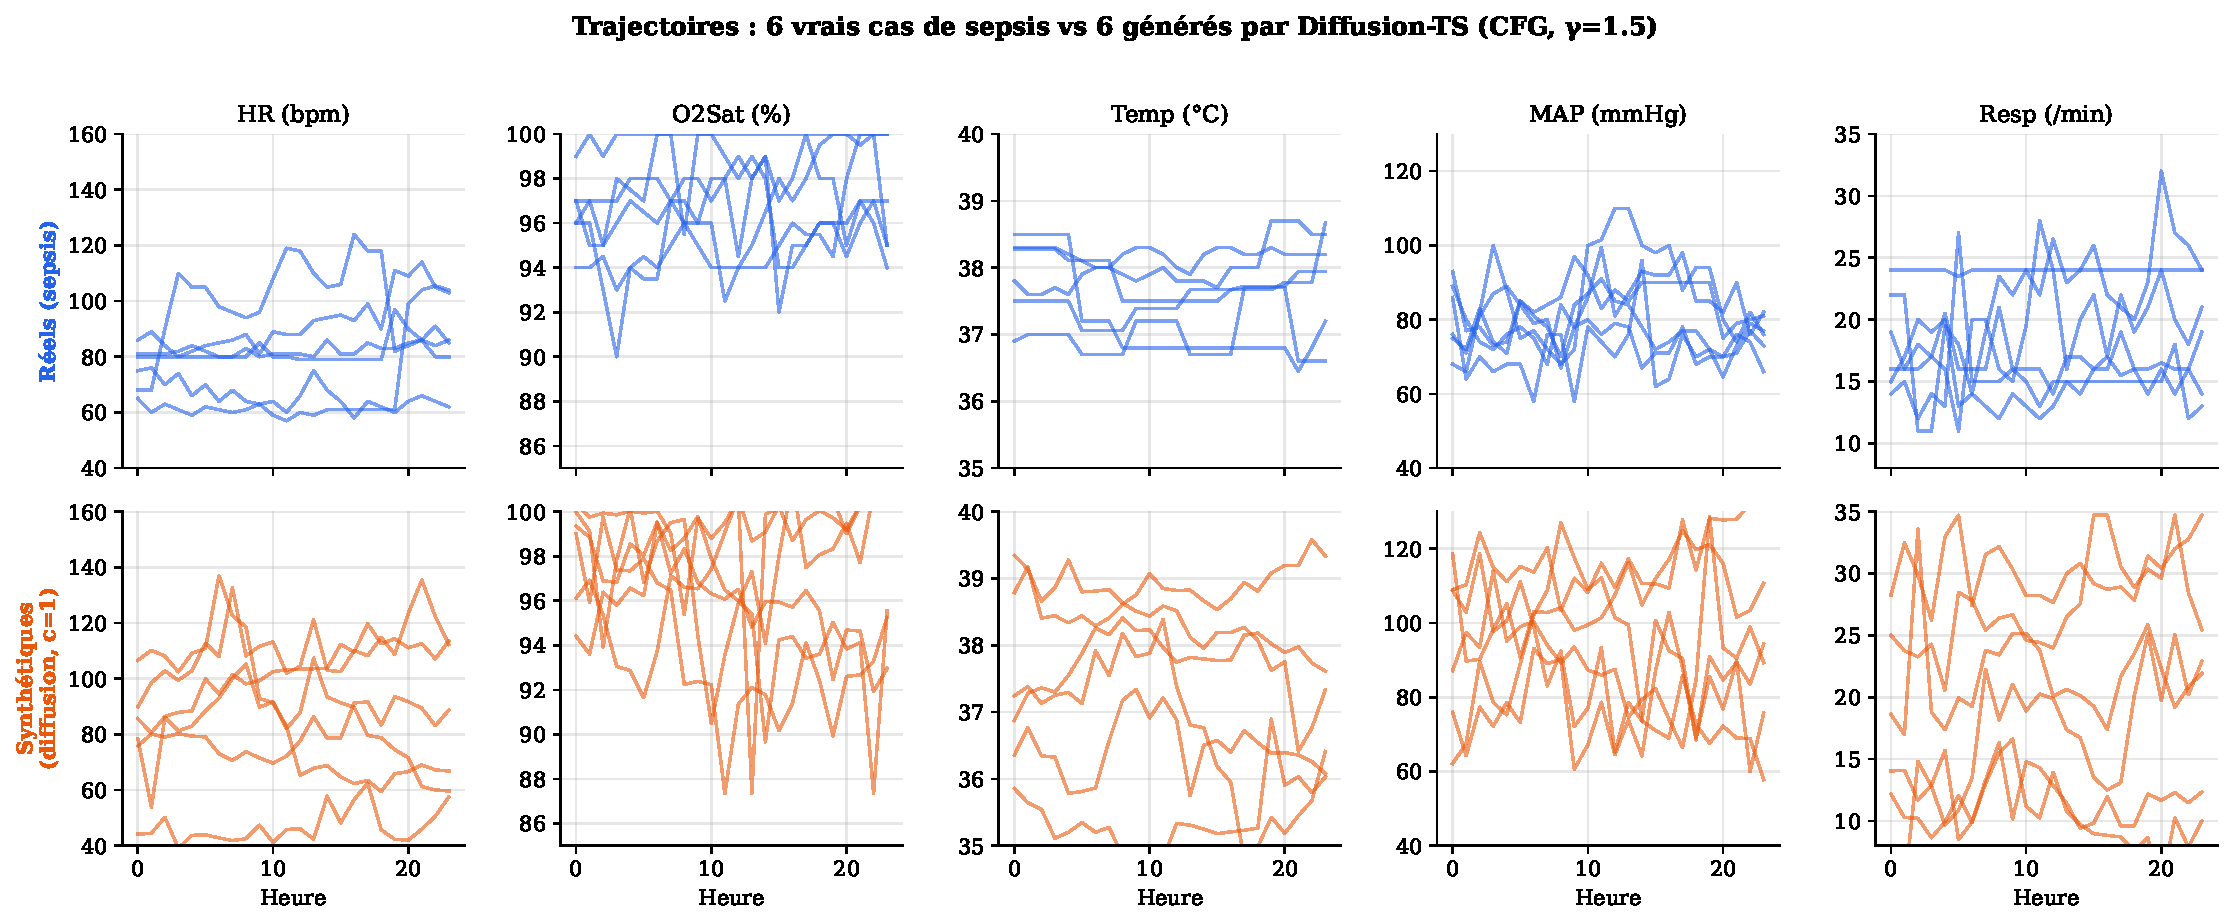
\includegraphics[width=\textwidth]{figures/synthetic_vs_real.pdf}
\caption{Trajectoires sur 24h de signes vitaux. \textbf{Haut (bleu) :} 6 patients réels
avec sepsis. \textbf{Bas (orange) :} 6 fenêtres synthétiques générées par Diffusion-TS
conditionné sur $c=1$ (DDIM, 50 pas, $\gamma=1.5$).}
\label{fig:traj}
\end{figure}

Les échantillons synthétiques reproduisent les grandes plages physiologiques
attendues (HR 50--130, Temp 35--41, MAP 50--130, etc.) ainsi que les variations
lentes d'amplitude réaliste (pas de discontinuités, pas de plateaux artificiels).
Les amplitudes sont parfois légèrement plus larges que sur les vrais patients,
reflet du coefficient de guidance $\gamma=1.5$ qui accentue le caractère
``pathologique'' au détriment de la diversité fine.

\begin{figure}[H]
\centering
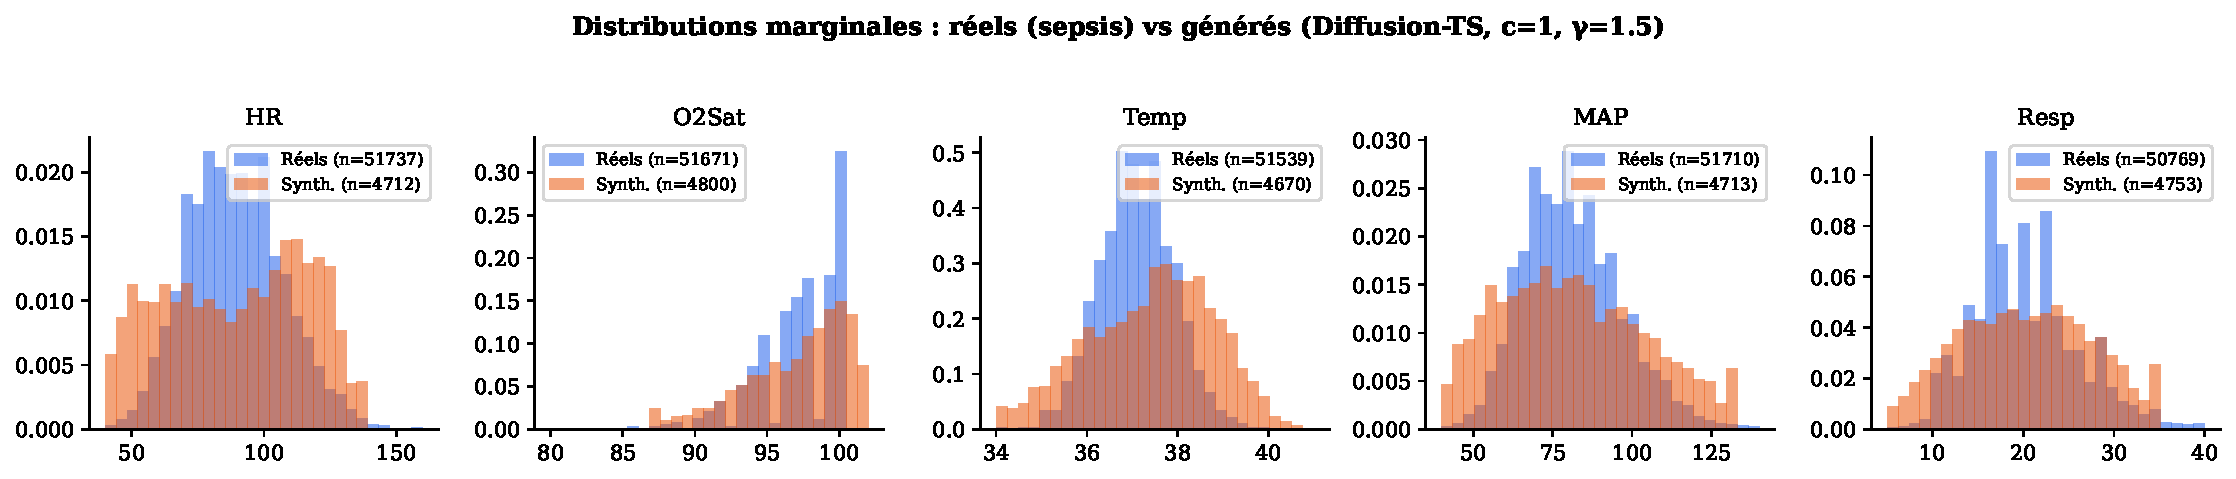
\includegraphics[width=\textwidth]{figures/distribution_real_vs_synth.pdf}
\caption{Distributions marginales des signes vitaux : valeurs réelles (sepsis,
$n \approx 2~157$ fenêtres $\times$ 24 pas) vs valeurs générées
(200 fenêtres synthétiques $\times$ 24 pas). Les distributions se recouvrent
largement, validant que les trajectoires synthétiques sont statistiquement
proches des vraies — condition nécessaire à un gain en classification.}
\label{fig:dist}
\end{figure}

Cette validation visuelle est essentielle : un gain de classification dû à des
échantillons aberrants ou trop éloignés de la distribution réelle ne
généraliserait pas. Ici le recouvrement des distributions confirme que la
diffusion apprend la bonne variété de données.

\subsection{Exemples qualitatifs (4 cas du test set)}

Pour illustrer concrètement la sortie du modèle, nous présentons quatre cas
représentatifs extraits du jeu de test, chacun choisi pour mettre en lumière
un comportement particulier (vrai positif confiant, vrai négatif confiant,
faux positif incertain, faux négatif silencieux). La table~\ref{tab:cases}
résume les plages observées des principaux signes vitaux sur la fenêtre 24h
et la sortie du classifieur.

\begin{table}[H]
\centering
\caption{Quatre cas extraits du test set (10\% de labels). Plages des signes vitaux
observés sur la fenêtre 24h, probabilité prédite par le modèle (moyenne sur 50
passes MC Dropout), variance associée, et décision binaire au seuil de Youden 0.018.
Les unités : HR en battements/min, MAP et SBP en mmHg, Temp en °C, Lactate en mmol/L.}
\label{tab:cases}
\renewcommand{\arraystretch}{1.3}
\resizebox{\textwidth}{!}{%
\begin{tabular}{lccccccccc}
\toprule
\textbf{Cas} & \textbf{HR} & \textbf{Temp} & \textbf{MAP} & \textbf{Lactate} &
\textbf{$y_{\text{vrai}}$} & \textbf{$P(\text{sepsis})$} & \textbf{Var MC ($\times 10^{-3}$)} &
\textbf{Décision} \\
\midrule
TP confiant      & 79--100  & 37.1--38.0 & 67--109 & non mesuré & sepsis & 0.419 & 1.07  & SEPSIS \checkmark \\
TN confiant      & 52--100  & 36.1--36.7 & 73--96  & non mesuré & sain   & 0.002 & 0.001 & non-sepsis \checkmark \\
\rowcolor{bestrow}
\textbf{FP incertain} & 86--\textbf{135} & 36.6--37.7 & 92$\to$\textbf{69} & non mesuré & sain & 0.728 & \textbf{19.5} & SEPSIS $\times$ \\
FN silencieux    & 62--86   & \textbf{35.0}--36.6 & 80--148 & 0.9--1.3   & sepsis & 0.013 & 0.12  & non-sepsis $\times$ \\
\bottomrule
\end{tabular}}
\end{table}

\paragraph{Interprétation clinique.}
Le \textbf{FP incertain} illustre l'apport principal du MC Dropout : le modèle
prédit à tort SEPSIS (la chute brutale de MAP de 92 à 69 mmHg associée à une
tachycardie marquée à 135 bpm évoque une instabilité hémodynamique compatible
avec un sepsis), \emph{mais} sa variance ($1.95 \times 10^{-2}$) est près de
\textbf{20 fois supérieure} à celle d'un TP confiant. Dans un système de surveillance
en USI, cette variance permettrait de classer cette alerte en \emph{"à vérifier"}
plutôt qu'en alarme automatique, économisant une intervention non nécessaire tout
en sollicitant le clinicien sur les cas réellement ambigus.

À l'inverse, le \textbf{FN silencieux} est plus problématique : le modèle rate
le sepsis (probabilité 0.013, sous le seuil 0.018) \emph{et} sa variance reste
faible — il ne sait pas qu'il se trompe. Ce cas, caractérisé par une hypothermie
atypique (35.0\,°C, à l'opposé du tableau classique fébrile) et un MAP large
mais variable, correspond à une présentation clinique trompeuse que la base
d'entraînement ne contient pas suffisamment. C'est la limite intrinsèque de
toute estimation d'incertitude basée uniquement sur la stochasticité interne
du modèle (incertitude épistémique) : elle ne capture pas l'incertitude
\emph{aléatoire} due aux données rares ou hors distribution.

\subsection{Ablation : impact du ratio de labels}

\begin{table}[H]
\centering
\caption{Performance en fonction du ratio de labels positifs utilisés pour le guidage
conditionnel. Le modèle de diffusion est ré-entraîné à chaque ratio.}
\renewcommand{\arraystretch}{1.3}
\begin{tabular}{crrrrr}
\toprule
\textbf{Ratio} & \textbf{Labels (+)} &
\textbf{AUROC}$\uparrow$ & \textbf{AUPRC}$\uparrow$ &
\textbf{F1}$\uparrow$ & \textbf{ECE}$\downarrow$ \\
\midrule
5\%  & 108  & 0.8642 & 0.1443 & 0.1410 & 0.0170 \\
10\% & 215  & 0.8679 & 0.1363 & 0.1139 & 0.0088 \\
25\% & 539  & 0.8669 & \textbf{0.1484} & 0.1153 & 0.0179 \\
\rowcolor{bestrow}
50\% & 1078 & 0.8684 & 0.1356 & 0.1228 & \textbf{0.0058} \\
\bottomrule
\end{tabular}
\end{table}

% ── 6. Analyse ─────────────────────────────────────────────────────────────────

\section{Analyse et Discussion}

\subsection{Apport de l'augmentation par diffusion}

La comparaison entre le Transformer vanilla (AUROC = 0.789) et notre méthode
(AUROC = 0.868) révèle un gain de \textbf{+7.9 points d'AUROC} dû exclusivement à
l'augmentation par génération conditionnelle. Ce résultat démontre que Diffusion-TS
produit des trajectoires patients synthétiques suffisamment réalistes pour entraîner
un classifieur robuste avec seulement 215 exemples positifs labellés.

\subsection{Comparaison avec les baselines supervisées}

Notre méthode surpasse le BiLSTM de \textbf{+2.7 pts AUROC} et de
\textbf{+25.5~\% relatif en AUPRC} (0.1363 vs 0.1086). L'AUPRC est la métrique
la plus pertinente pour les datasets déséquilibrés car elle est insensible à
l'abondance de vrais négatifs. Le score d'utilité PhysioNet est le plus
discriminant : $-0.080$ pour notre méthode contre $-0.165$ pour le BiLSTM
(2$\times$ meilleur), traduisant un meilleur compromis sensibilité/spécificité
au seuil opérationnel.

Le F1 du BiLSTM (0.1252) est légèrement supérieur au nôtre (0.1139) : un modèle
entraîné sur données synthétiques a une frontière de décision plus diffuse, ce qui
pénalise marginalement le F1 à seuil fixe.

\subsection{Qualité de la calibration et incertitude}

L'ECE de \textbf{0.009} indique une très bonne calibration, propriété essentielle
en milieu clinique. La corrélation incertitude--erreur de \textbf{0.258} confirme
l'utilité du MC Dropout : la variance sur les prédictions incorrectes est
\textbf{6.6 fois plus élevée} que sur les correctes ($1.39\times10^{-3}$ vs
$2.12\times10^{-4}$).

\subsection{Robustesse au ratio de labels}

Le résultat le plus frappant de l'ablation est la \textbf{stabilité remarquable de l'AUROC}
à travers tous les ratios : la variation totale n'est que de 0.004 points (0.8642 à 0.8684).
Cela s'explique par l'architecture semi-supervisée : le modèle de diffusion apprend la
distribution générale des trajectoires patients sur \emph{toutes} les données sans supervision,
et le guidage conditionnel ne sert qu'à orienter la génération synthétique. Avec seulement
\textbf{108 exemples positifs labellés (5\%)}, le système atteint déjà AUROC = 0.864.

L'AUPRC culmine à 25\% (0.1484), suggérant que le rapport signal/bruit dans les données
synthétiques générées est optimal à ce ratio. En dessous (5--10\%), les synthétiques sont
moins fidèles faute de supervision ; au-dessus (50\%), le surplus de labels n'apporte pas
de gain car la distribution est déjà bien capturée.

L'ECE est minimale à 50\% (0.0058) — la configuration la mieux calibrée — tandis qu'à
25\% on observe le plus mauvais ECE (0.0179) malgré la meilleure AUPRC. La calibration
bayésienne du MC Dropout n'évolue donc pas de façon monotone avec le ratio de labels,
mais reste partout inférieure à 0.02, ce qui demeure cliniquement acceptable.

\subsection{Entraînement et early stopping}

L'évolution de l'AUROC de validation a révélé un sur-apprentissage dès l'epoch~9
(AUROC = 0.8521 à l'epoch~8, puis déclin vers 0.760 à l'epoch~50). L'early stopping
avec patience = 10 a permis de sauvegarder le meilleur modèle automatiquement.
Ce comportement s'explique par la présence de données synthétiques dans le jeu
d'entraînement augmenté : le modèle finit par mémoriser leurs patterns plutôt que
les patterns cliniques réels.

\subsection{Score d'utilité clinique PhysioNet}

Le score de \textbf{$-0.080$} est très proche de zéro (vs $-1.97$ avec seuil par défaut
de 0.5). Le seuil optimal de 0.0178 reflète le déséquilibre asymétrique de la fonction
de coût clinique : pénalité FN = $-2.0$, pénalité FP = $-0.05$.

\subsection{Limitations}

\begin{enumerate}
    \item \textbf{AUPRC modeste (0.136)} : les meilleures solutions du challenge
    PhysioNet 2019 atteignaient 0.3--0.5 avec accès à l'intégralité des labels.
    \item \textbf{Diffusion sous-entraînée} : 100 epochs suffisent pour faire converger
    la loss mais pas pour générer des échantillons optimaux. Un entraînement à
    200+ epochs améliorerait la qualité des synthétiques.
    \item \textbf{Score d'utilité simplifié} : nous utilisons une approximation du score
    PhysioNet 2019 (TP/FP/FN/TN constants par fenêtre) au lieu de la version officielle
    par-patient avec décroissance temporelle (\texttt{dt\_early}, \texttt{dt\_optimal},
    \texttt{dt\_late}). Les valeurs absolues ne sont donc pas directement comparables
    aux scores du challenge ; les comparaisons inter-méthodes au sein de ce rapport
    restent cohérentes car toutes utilisent la même formule.
\end{enumerate}

% ── 7. Conclusion ──────────────────────────────────────────────────────────────

\section{Conclusion}

Ce projet démontre la faisabilité de l'adaptation de Diffusion-TS à la prédiction
précoce du sepsis dans un cadre semi-supervisé avec incertitude bayésienne.
Les trois contributions sont validées expérimentalement :

\begin{enumerate}
    \item \textbf{L'augmentation par diffusion améliore significativement la classification}
    (+7.9 pts AUROC vs Transformer vanilla, +2.7 pts vs BiLSTM supervisé).
    \item \textbf{Le MC Dropout produit des scores d'incertitude utiles} : variance
    6.6$\times$ plus élevée sur les erreurs, ECE = 0.009.
    \item \textbf{La diffusion surpasse les GAN-based} en stabilité d'entraînement,
    sans effondrement de mode ni oscillation de la loss.
\end{enumerate}

Code source, tests (76 tests, 100~\% de réussite) et instructions de reproduction :
\url{https://github.com/BigYellowData/diffusion-ts-sepsis}

% ── Références ─────────────────────────────────────────────────────────────────

\newpage

\begin{thebibliography}{9}

\bibitem{diffusion-ts}
Yuan, X. \& Qiao, Y. (2024).
\textit{Diffusion-TS: Interpretable Diffusion for General Time Series Generation}.
ICLR 2024.

\bibitem{physionet2019}
Reyna, M.A. et al. (2020).
\textit{Early Prediction of Sepsis from Clinical Data: The PhysioNet/Computing in
Cardiology Challenge 2019}. Critical Care Medicine.

\bibitem{gal2016dropout}
Gal, Y. \& Ghahramani, Z. (2016).
\textit{Dropout as a Bayesian Approximation: Representing Model Uncertainty in Deep Learning}.
ICML 2016.

\bibitem{nichol2021improved}
Nichol, A. \& Dhariwal, P. (2021).
\textit{Improved Denoising Diffusion Probabilistic Models}. ICML 2021.

\bibitem{hirnschall2025}
Hirnschall, D. (2025).
\textit{Semi-Supervised Bayesian GANs with Log-Signatures for Uncertainty-Aware
Credit Card Fraud Detection}. arXiv.

\bibitem{morrill2020}
Morrill, J. et al. (2020).
\textit{Utilization of the Signature Method to Identify the Early Onset of Sepsis
from Multivariate Physiological Time Series}. Critical Care Medicine, 48(10).

\end{thebibliography}

\end{document}
